\documentclass[a4paper,12pt]{report}
\usepackage{a4wide}

%\documentclass[a5paper,10pt]{book}
%\usepackage[top=23mm, bottom=18mm, left=15mm, right=25mm]{geometry}
%\geometry{papersize={170mm,220mm}}


\usepackage[utf8x]{inputenc}
\usepackage[danish]{babel}

\usepackage{xr-hyper} %Externe hyper-ref
\usepackage[colorlinks=true, hyperindex=true, linkcolor=minmblaa, citecolor=minmblaa, urlcolor=minmblaa]{hyperref}
\hypersetup{colorlinks=true,filecolor=minmblaa,bookmarksnumbered=true} %Til hyperreferencer. Referencer med farver
\usepackage{needspace} % giver mulighed for at kræve at der skal være et antal tomme linier på siden før ellers indsættes et sideskift.
\usepackage{framed} %Bokse
\usepackage{wrapfig}

\usepackage{amsmath,amsfonts,amssymb,amsthm,mathtools} %Matematikpakker

\setlength{\parindent}{0mm} %Ingen Indhak i første linje i afsnit

\usepackage{color} %Farvepakke

\usepackage{array}
\usepackage{colortbl}
\usepackage{multirow} %Til at flette rækker i tabeller.

\usepackage{verbatim,mhchem}



	% DOWNLOAD FRA: http://sarovar.org/frs/?group_id=52&release_id=97
	% Læg i directory for hoved TEX fil
%\usepackage[draft]{pdfdraftcopy}
%\draftstring{Licens: Kasper Langt Mellemnavn Skårhøj}
%\draftfontsize{30}
	%\draftfontfamily{hlh}
	%\draftangle{45}
	%\definecolor{mycolor}{rgb}{.825,.855,1}
	%\draftcolor{mycolor}
	%\draftfontattrib



% = Sidehoved =
\usepackage{fancyhdr}
\pagestyle{fancy}
\renewcommand{\sectionmark}[1]{\markright{\protect\titlegraphic{dturoed}\textcolor{dtugraa}{\thesection~\MakeUppercase{#1}}}} % \thesection.\
\fancyhead{}
\fancyfoot{}
\fancyhead[R]{\titlefont\thepage}
\fancyhead[C]{}
\fancyhead[L]{\titlefont \small eNote \MakeUppercase{~\thechapter}~\hspace*{1ex}\rightmark}
\renewcommand\headrulewidth{0pt}
\fancypagestyle{plain}{\fancyfoot[C]{}}% {\titlefont\footnotesize\thepage}}
\setlength{\headheight}{15pt}


% = Længder
%\newlength{\envtblsep}\setlength{\envtblsep}{1\FrameSep}
\newlength{\obsl}\setlength{\obsl}{\textwidth-1.2cm-13.2pt}

% Includes:

% =     Fonts (select one)    =
\usepackage{mathpazo}\linespread{1.05} % Palatino needs more leading (space between lines)
\usepackage{bm} % bold math, must be loaded after the fontpackages

% % Til overskrifter
\DeclareTextFontCommand{\th}{\fontencoding{T1}\fontfamily{phv}\fontseries{b}\selectfont}
\newcommand\titlefont{\fontencoding{T1}\fontfamily{phv}\selectfont}


% =     PGF grafik      =
\usepackage{tikz}
\newcommand\titlegraphic[1]{%
\tikz[baseline] %
\draw[thick,color=#1]
(0pt  ,-0.25em) -- (0pt  ,0.85em)
(2.5pt,-0.25em) -- (2.5pt,0.85em)
(5pt  ,-0.25em) -- (5pt  ,0.85em)
(7.5pt,-0.25em) -- (7.5pt,0.85em);\hspace*{0.8ex} %
}

\newcommand\titlegraphicwide[1]{%
\tikz[baseline] %
\draw[line width=0.8mm,color=#1]
(0pt  ,-0.25em) -- (0pt  ,0.85em)
(4.5pt,-0.25em) -- (4.5pt,0.85em)
(9pt  ,-0.25em) -- (9pt  ,0.85em)
(13.5pt,-0.25em) -- (13.5pt,0.85em);\hspace*{0.8ex} %
}


% =      Title Layout      =
\usepackage{titlesec}
\makeatletter
\titleformat{\chapter}
	[display] % Shape
	{\titlefont\Huge\flushleft} % Title and label format
	{\titlefont\LARGE\bfseries \titlegraphicwide{dturoed}\textcolor{dtugraa}{\@chapapp~\thechapter}} % label
	{0.9em} % label/title separation
	{} % before code
	[] % after code
\makeatother
\titleformat{\section}
	[hang] % Shape
	{\titlefont\Large\flushleft} % Title and label format
	{\thesection} % label
	{0.9em} % label/title separation
	{} % before code
	[] % after code
\titleformat{\subsection}
	[hang] % Shape
	{\titlefont\large} % Title and label format
	{\thesubsection} % label
	{0.9em} % label/title separation
	{} % before code
	[] % after code
\titlespacing{\subsection}{0pt}{*6}{*1.5}
\titleformat{\subsubsection}
	[hang] % Shape
	{\titlefont} % Title and label format
	{\thesubsubsection} % label
	{0.9em} % label/title separation
	{} % before code
	[] % after code



% = Farver
\definecolor{dturoed}{rgb}{0.6, 0.0, 0.0}
\definecolor{dtugraa}{rgb}{0.5, 0.5, 0.5}	% Lidt mørkere. Korrekt = 0.4
\definecolor{mingroenstreg}{rgb}{0.4,0.8,0}	% Sekundærfarve 14 : 102/204/0	(Forårsgrøn) -> Eksempler
\definecolor{mingroen}{rgb}{0.32,0.64,0}		% Sekundærfarve 14, 80% mørkere (tekst)
\definecolor{minorangestreg}{rgb}{1,0.6,0}		% Sekundærfarve 1 : 255/153/0	(Orange) -> Opgaver
\definecolor{minorange}{rgb}{0.8,0.48,0}		% Sekundærfarve 1 , 80% mørkere (tekst)

\definecolor{minblaa}{rgb}{0.2,0.4,0.8}	% Sekundærfarve 13 , 51/102/204 	( Blå -> Definitioner etc)
\definecolor{minmblaa}{rgb}{0.16,0.32,0.64}	% Sekundærfarve 13 , 80% mørkere (tekst)
\definecolor{thmbackground}{rgb}{0.97,.97, 0.99}	% Farve 13 - lys baggrund

\definecolor{mingraastreg}{rgb}{.5,.5,.5}
\definecolor{hvadbackground}{rgb}{0.97,.97, 0.97}
\definecolor{sumgul}{rgb}{1,1,.8}

\definecolor{hjmopgfarve}{rgb}{.96,1,.96}


% = Counter
\newcounter{evncount}[chapter]
\setcounter{evncount}{0}
\renewcommand{\theevncount}{\thechapter.\arabic{evncount}}
\renewcommand{\theequation}{\thechapter-\arabic{equation}}


% = Eksempler = example =
\newenvironment{example}[1][]{
	\refstepcounter{evncount}
	\setlength{\obsl}{\textwidth-1.2cm-13.2pt-9pt} % fix width of the info envirnment%
	\def\FrameCommand{ 
		\textcolor{mingroenstreg}{\vrule width 4pt} 
		\hspace{5pt} 
	}%
	\MakeFramed{\advance\hsize-\width \FrameRestore}%
	\needspace{3\baselineskip}
	\titlegraphic{mingroen}
	\textcolor{mingroen}{
		\th{Eksempel \theevncount \hspace*{5mm} #1}
	} 
	\vspace*{3mm}%
	\begin{small}
	\par
}
{
	\end{small}
	\endMakeFramed
}


% = Opgaver = exercise =
\newenvironment{exercise}[1][]{
	\refstepcounter{evncount}
	\setlength{\obsl}{\textwidth-1.2cm-13.2pt-9pt}% fix width of the info envirnment%
	\def\FrameCommand{
		\textcolor{minorangestreg}{\vrule width 4pt}
		\hspace{5pt}
	}%
	\MakeFramed{\advance\hsize-\width \FrameRestore}%
	\needspace{3\baselineskip}
	\titlegraphic{minorange}
	\textcolor{minorange}{
		\th{Opgave \theevncount \hspace*{5mm} #1}
	} 
	\vspace*{3mm}%
	\begin{small}
	\par
}
{
	\end{small}
	\endMakeFramed
}


% = Bevis
\newenvironment{bevis}{
	\setlength{\obsl}{\textwidth-1.2cm-13.2pt-9pt} % fix width of the info envirnment%
	\def\FrameCommand{
		\textcolor{mingraastreg}{\vrule width 4pt} 
		\hspace{5pt}
	}%
	\MakeFramed{\advance\hsize-\width \FrameRestore}%
	\needspace{3\baselineskip}
	\titlegraphic{black}
	\textcolor{black}{
		\th{Bevis}
	}
	\vspace*{3mm}%
	\begin{small}
	\par
}
{
	\bevisslut 
	\end{small}
	\endMakeFramed
}


% = Definition =
\newenvironment{definition}[1][]{
	\vspace{4mm}
	\pagebreak[1]
	\setlength{\obsl}{\textwidth-1.2cm-2\FrameSep-13.2pt}%
	\def\FrameCommand{
		\fboxsep=\FrameSep\fcolorbox{minblaa}{thmbackground}
	}
	\begin{minipage}{\textwidth}
	\MakeFramed{\advance\hsize-\width\FrameRestore}
	\refstepcounter{evncount}
	\titlegraphic{minblaa}
	\textcolor{minmblaa}{
		\th{Definition \theevncount \hspace*{5mm} #1}
	}
	\vspace*{3mm}
	\par
}
{
	\endMakeFramed 
	\end{minipage}
	\vspace{4mm}
}


% = Theorem =
\newenvironment{theorem}[1][]{
	\vspace{4mm}
	\pagebreak[1]%
	\setlength{\obsl}{\textwidth-1.2cm-2\FrameSep-13.2pt}%
	\def\FrameCommand{
		\fboxsep=\FrameSep\fcolorbox{minblaa}{thmbackground}
	}%
	\begin{minipage}{\textwidth}
	\MakeFramed{\advance\hsize-\width\FrameRestore}%
	\refstepcounter{evncount}
	\titlegraphic{minblaa}
	\textcolor{minmblaa}{
		\th{Sætning \theevncount \hspace*{5mm} #1}
	}
	\vspace*{3mm}
	\par
}
{
	\endMakeFramed 
	\end{minipage}
	\vspace{4mm}
}


% = Lemma =
\newenvironment{lemma}[1][]{
	\vspace{4mm}
	\pagebreak[1]
	\setlength{\obsl}{\textwidth-1.2cm-2\FrameSep-13.2pt}%
	\def\FrameCommand{
		\fboxsep=\FrameSep \fcolorbox{minblaa}{thmbackground}
	}
	\begin{minipage}{\textwidth} 
	\MakeFramed{\advance\hsize-\width \FrameRestore}
	\refstepcounter{evncount}
	\titlegraphic{minblaa}
	\textcolor{minmblaa}{
		\th{Hjælpesætning \theevncount \hspace*{5mm} #1}
	}
	\vspace*{3mm}
	\par
}
{
	\endMakeFramed 
	\end{minipage}
	\vspace{4mm}
}


% = Corollary =
\newenvironment{corollary}[1][]{
	\vspace{4mm}
	\pagebreak[1]
	\setlength{\obsl}{\textwidth-1.2cm-2\FrameSep-13.2pt}%
	\def\FrameCommand{
		\fboxsep=\FrameSep \fcolorbox{minblaa}{thmbackground}
	}
	\begin{minipage}{\textwidth} 
	\MakeFramed{\advance\hsize-\width \FrameRestore}
	\refstepcounter{evncount}
	\titlegraphic{minblaa}
	\textcolor{minmblaa}{
		\th{Følgesætning \theevncount \hspace*{5mm} #1}
	}
	\vspace*{3mm}
	\par
}
{
	\endMakeFramed 
	\end{minipage}
	\vspace{4mm}
}


% = Metode = method
\newenvironment{method}[1][]{
	\vspace{4mm}
	\pagebreak[1]
	\setlength{\obsl}{\textwidth-1.2cm-2\FrameSep-13.2pt}%
	\def\FrameCommand{
		\fboxsep=\FrameSep \fcolorbox{black}{hvadbackground}
	}
	\begin{minipage}{\textwidth} 
	\MakeFramed{\advance\hsize-\width \FrameRestore}
	\refstepcounter{evncount}
	\titlegraphic{black}
	\textcolor{black}{
		\th{Metode \theevncount \hspace*{5mm} #1}
	}
	\vspace*{3mm}
	\par
}
{
	\endMakeFramed
	\end{minipage}
	\vspace{4mm}
}


% = Forklaring = explain =
\newenvironment{explain}[1][]{
	\vspace{4mm}
	\pagebreak[1]
	\setlength{\obsl}{\textwidth-1.2cm-2\FrameSep-13.2pt}%
	\def\FrameCommand{
		\fboxsep=\FrameSep \fcolorbox{black}{hvadbackground}
	}
	\MakeFramed{\advance\hsize-\width \FrameRestore}
	\refstepcounter{evncount}
	\titlegraphic{black}
	\textcolor{black}{
		\th{Forklaring \theevncount \hspace*{5mm} #1}
	}
	\vspace*{3mm}
	\par
}
{
	\endMakeFramed
	\vspace{4mm}
}


% = Bemærkning = remark =
\newenvironment{remark}[1][]{
	\vspace{4mm}
	\pagebreak[1]
	\setlength{\obsl}{\textwidth-1.2cm-2\FrameSep-13.2pt}%
	\def\FrameCommand{
		\fboxsep=\FrameSep \fcolorbox{black}{hvadbackground}
	}
	\begin{minipage}{\textwidth} 
	\MakeFramed{\advance\hsize-\width \FrameRestore}
	\refstepcounter{evncount}
	\titlegraphic{black}
	\textcolor{black}{
		\th{Bemærkning \theevncount \hspace*{5mm} #1}
	}
	\vspace*{3mm}
	\par
}
{
	\endMakeFramed 
	\end{minipage}
	\vspace{4mm}
}







% = OBS! = obs =
\newenvironment{obs}{\vspace{4mm}\par%
\begin{tabular}{m{1.2cm}<{\hspace*{2mm}}@{}|m{\obsl}@{}}\hspace*{-4pt}\raggedleft
\includegraphics[width=1.1cm]{../Strukturfiler/FIGS/Alert01} & \begin{minipage}{\obsl}}{\end{minipage}\\ \end{tabular}\vspace{4mm}\par}


% = INFO = info =
\newenvironment{info}{\vspace{4mm}\par%
\begin{tabular}{m{1.2cm}<{\hspace*{2mm}}@{}|m{\obsl}@{}}\hspace*{-4pt}\raggedleft
\includegraphics[width=1.1cm]{../Strukturfiler/FIGS/Info01} & \begin{minipage}{\obsl}}{\end{minipage}\\ \end{tabular}\vspace{4mm}\par}


% = THINK= think =
\newenvironment{think}{\vspace{4mm}\par%
\begin{tabular}{m{1.2cm}<{\hspace*{2mm}}@{}|m{\obsl}@{}}\hspace*{-4pt}\raggedleft
\includegraphics[width=0.7cm]{../Strukturfiler/FIGS/ChessPiece} & \begin{minipage}{\obsl}}{\end{minipage}\\ \end{tabular}\vspace{4mm}\par}


% = AHA= aha =
\newenvironment{aha}{\vspace{4mm}\par%
\begin{tabular}{m{1.2cm}<{\hspace*{2mm}}@{}|m{\obsl}@{}}\hspace*{-4pt}\raggedleft
\includegraphics[width=1.1cm]{../Strukturfiler/FIGS/Think} & \begin{minipage}{\obsl}}{\end{minipage}\\ \end{tabular}\vspace{4mm}\par}


% = BUILDUP= build =
\newenvironment{build}{\vspace{4mm}\par%
\begin{tabular}{m{1.2cm}<{\hspace*{2mm}}@{}|m{\obsl}@{}}\hspace*{-4pt}\raggedleft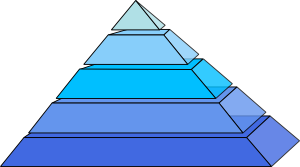
\includegraphics[width=1.1cm]{../Strukturfiler/FIGS/BluePyramid} & \begin{minipage}{\obsl}}{\end{minipage}\\ \end{tabular}\vspace{4mm}\newline}


% = Forudsætning = basis
\newenvironment{basis}{\begin{flushleft} \begin{itshape} }{\end{itshape} \end{flushleft}}


% = Opsummering =
\newenvironment{summary}{\clearpage\pagecolor{sumgul}\section{Opsummering}}{\newpage\pagecolor{white}}











% = Counter
\newcounter{opgavecount}[section]
\setcounter{opgavecount}{0}
\newcounter{spgcount}[opgavecount]
\setcounter{spgcount}{0}
\renewcommand{\thespgcount}{\alph{spgcount})}



% = EXERCISE = (DIVIDER)

\newcommand{\exercisebegin}[1][]{\bigskip\needspace{3\baselineskip}\refstepcounter{opgavecount}\titlegraphic{mingroen}\textcolor{mingroen}{\th{Opgave \theopgavecount \hspace*{1cm} #1}}\medskip\par}

% = QUIZEXERCISE = (DIVIDER)

\newcommand{\quizexercisebegin}[1][]{\bigskip\needspace{3\baselineskip}\refstepcounter{opgavecount}\titlegraphic{mingroen}\textcolor{mingroen}{\th{Quiz-Opgave \theopgavecount \hspace*{1cm} #1}}\medskip\par}

% = QUESTION =

\newenvironment{question}{\refstepcounter{spgcount}\begin{itemize}\item[\thespgcount]}{\end{itemize}\hspace*{\fill}}

% = VINK =

\newenvironment{vink}{\begin{tabular}{m{.9cm}<{\hspace*{2mm}}@{}|m{\obsl}@{}}\hspace*{-4pt}\raggedleft
\includegraphics[width=.9cm]{../Strukturfiler/FIGS/Think} & \begin{minipage}{\obsl}}{\end{minipage}\\ \end{tabular}\medskip\\}
	
% = FACIT =

\newenvironment{facit}{\begin{tabular}{m{.9cm}<{\hspace*{2mm}}@{}|m{\obsl}@{}}\hspace*{-4pt}\raggedleft
\includegraphics[width=.9cm]{../Strukturfiler/FIGS/Check} & \begin{minipage}{\obsl}}{\end{minipage}\\ \end{tabular}\medskip\\}








\newcommand{\afsnit}[1]{\bigskip\th{\titlegraphic{mingroen}\textcolor{mingroen}{#1}} \\ \rule[7pt]{.4\textwidth}{1pt} \vspace*{-2.5mm}\par}

% (DIVIDER):
\newcommand{\ugedagdatotitel}[4]{\pagebreak[4]\section{Semesteruge #1 -- #2 Dag \hspace*{1mm} (#3)} \vspace*{-4mm} \rule[5pt]{\textwidth}{1pt}\vspace*{-2.5mm} \begin{center}\large{\th{#4}}\end{center} \fancyhead[C]{\th{Semesteruge #1}}}

\newenvironment{skema}[1]{\definecolor{shadecolor}{rgb}{0.96,.98, 1.0} \setlength{\FrameSep}{6pt} \renewcommand{\FrameHeightAdjust}{10pt} \vspace*{-4pt}\begin{shaded} \begin{tabular}{#1}}{\end{tabular} \end{shaded} \vspace*{-7pt}}


% ========================

% MAKROER

%\newenvironment{matr}[1][]{\hspace*{-.8mm}\left[\hspace*{-1mm}\begin{array}{#1}}{\end{array}\hspace*{-1mm}\right]\hspace*{-.8mm}}
\newcommand{\bevisslut}{\begin{scriptsize} \begin{flushright} $ \blacksquare $ \end{flushright} \end{scriptsize}}

\newcommand{\tref}[2]{\hyperref[#1]{#2 \ref*{#1}}}
\newcommand{\thref}[2]{\hyperref[#1]{#2}}

\newcommand{\refA}[1]{\colorbox{yellow}{\ref{#1}}}
\newcommand{\hrefA}[2]{\colorbox{yellow}{\href{#1}{#2}}}
\newcommand{\trefA}[2]{\colorbox{yellow}{\hyperref[#1]{#2 \ref*{#1}}}}
\newcommand{\threfA}[2]{\colorbox{yellow}{\hyperref[#1]{#2}}}

\newenvironment{matr}[1]{\hspace*{-.8mm}\begin{bmatrix}\hspace*{-1mm}\begin{array}{#1}}{\end{array}\hspace*{-1mm}\end{bmatrix}\hspace*{-.8mm}}
\newcommand{\transp}{\hspace*{-.6mm}^{\top}}

\newcommand{\maengde}[2]{\left\lbrace \hspace*{-1mm} \begin{array}{c|c} #1 & #2 \end{array} \hspace*{-1mm} \right\rbrace}

\newenvironment{eqnalign}[1]{\setlength{\arraycolsep}{1.3pt}\begin{equation}\begin{array}{#1}}{\end{array}\end{equation}\par}
\newcommand{\eqnl}{\setlength{\arraycolsep}{1.3pt}}

\newcommand{\matind}[3]{{_\mathrm{#1}\mathbf{#2}_\mathrm{#3}}}
\newcommand{\vekind}[2]{{_\mathrm{#1}\mathbf{#2}}}
\newcommand{\jac}[2]{{\mathrm{Jacobi}_\mathbf{#1} (#2)}}
\newcommand{\diver}[2]{{\mathrm{div}\mathbf{#1} (#2)}}
\newcommand{\rot}[1]{{\mathbf{rot}\mathbf{(#1)}}}

\newcommand{\am}{\mathrm{am}}
\newcommand{\gm}{\mathrm{gm}}
\newcommand{\E}{\mathrm{E}}
\newcommand{\Span}{\mathrm{span}}
\newcommand{\mU}{\mathbf{U}}

\newcommand{\ms}{\medskip\\}
\newcommand{\bs}{\bigskip\\}

\newcommand{\mA}{\mathbf{A}}
\newcommand{\mB}{\mathbf{B}}
\newcommand{\mC}{\mathbf{C}}
\newcommand{\mD}{\mathbf{D}}
\newcommand{\mE}{\mathbf{E}}
\newcommand{\mF}{\mathbf{F}}
\newcommand{\mK}{\mathbf{K}}
\newcommand{\mI}{\mathbf{I}}
\newcommand{\mM}{\mathbf{M}}
\newcommand{\mN}{\mathbf{N}}
\newcommand{\mQ}{\mathbf{Q}}
\newcommand{\mT}{\mathbf{T}}
\newcommand{\mV}{\mathbf{V}}
\newcommand{\mW}{\mathbf{W}}
\newcommand{\mX}{\mathbf{X}}
\newcommand{\ma}{\mathbf{a}}
\newcommand{\mb}{\mathbf{b}}
\newcommand{\mc}{\mathbf{c}}
\newcommand{\md}{\mathbf{d}}
\newcommand{\me}{\mathbf{e}}
\newcommand{\mn}{\mathbf{n}}
\newcommand{\mr}{\mathbf{r}}
\newcommand{\mv}{\mathbf{v}}
\newcommand{\mw}{\mathbf{w}}
\newcommand{\mx}{\mathbf{x}}
\newcommand{\mxb}{\mathbf{x_{bet}}}
\newcommand{\my}{\mathbf{y}}
\newcommand{\mz}{\mathbf{z}}
\newcommand{\reel}{\mathbb{R}}
\newcommand{\mL}{\bm{\Lambda}} %Lambda-matrix
\newcommand{\mnul}{\bm{0}}
\newcommand{\trap}[1]{\mathrm{trap}(#1)}
\newcommand{\Det}{\operatorname{Det}}
\newcommand{\adj}{\operatorname{adj}}
\newcommand{\Ar}{\operatorname{Areal}}
\newcommand{\Vol}{\operatorname{Vol}}
\newcommand{\Rum}{\operatorname{Rum}}
\newcommand{\diag}{\operatorname{\bf{diag}}}
\newcommand{\bidiag}{\operatorname{\bf{bidiag}}}
\newcommand{\spanVec}[1]{\mathrm{span}\{#1\}}
\newcommand{\Div}{\operatorname{Div}}
\newcommand{\Rot}{\operatorname{\mathbf{Rot}}}

\newcommand{\Jac}{\operatorname{Jacobi}}
\newcommand{\Tan}{\operatorname{Tan}}
\newcommand{\Ort}{\operatorname{Ort}}
\newcommand{\Flux}{\operatorname{Flux}}
\newcommand{\Cmass}{\operatorname{Cm}}
\newcommand{\Imom}{\operatorname{Im}}
\newcommand{\Pmom}{\operatorname{Pm}}
\newcommand{\IS}{\operatorname{I}}
\newcommand{\IIS}{\operatorname{II}}
\newcommand{\IIIS}{\operatorname{III}}
\newcommand{\Le}{\operatorname{L}}
\newcommand{\app}{\operatorname{app}}
\newcommand{\M}{\operatorname{M}}
\newcommand{\re}{\mathrm{Re}}
\newcommand{\im}{\mathrm{Im}}

\newcommand{\compl}{\mathbb{C}} %de komplekse tal
\newcommand{\e}{\mathrm{e}} %eksponentialfunktionen. lodret 'e', og altså ikke kursiv ligesom andre bogstaver.





% Medialink: SCREEN: (QRcode) + thumbnail image + link på kodenummer (til qr.dtu.dk)
\newcommand{\onlinemedia}[3]{
	\begin{wrapfigure}{r}{3.2cm} 
		\vspace{-30pt} 
		\vspace{#1pt} 
		\begin{flushright} 
			\includegraphics[width=3cm]{qr/#2.png} 
			\tiny 
			\href{http://qr.dtu.dk/#2}{#2: #3}
			\normalsize  
		\end{flushright} 
		\vspace{-10pt} 
	\end{wrapfigure}
}
\newcommand{\onlinemediathumb}[3]{
	\begin{wrapfigure}{r}{3.2cm} 
		\vspace{-30pt} 
		\vspace{#1pt} 
		\begin{flushright} 
			\includegraphics[width=3cm]{qr/#2.png} 
			\includegraphics[width=3cm]{qr/#2_thumb.png} 
			\tiny 
			\href{http://qr.dtu.dk/#2}{#2: #3}
			\normalsize  
		\end{flushright} 
		\vspace{-10pt} 
	\end{wrapfigure}
}



% Index:
\usepackage{makeidx}
\makeindex
\newcommand\ind[2]{\index{#1}\textbf{\textit{\textcolor{black}{#2}}}}

% ###SERVER_EXCLUDE_BEGIN###
\externaldocument[NUID17-]{../../enoten/TN01-Talrum/Talrum}
\externaldocument[NUID1-]{../../enoten/TN02-Ligningssystemer/TNdriver}
\externaldocument[NUID2-]{../../enoten/TN03-Matricer_og_Matrixalgebra/Matricer_og_matrixalgebra}
\externaldocument[NUID3-]{../../enoten/TN04-Kvadratiske_matricer/TNdriver}
\externaldocument[NUID11-]{../../enoten/TN05-Determinanter/Determinanter}
\externaldocument[NUID12-]{../../enoten/TN06-GeometriskeVektorer/GeometriskeVektorer}
\externaldocument[NUID18-]{../../enoten/TN07-Vektorrum/VektorRum}
\externaldocument[NUID21-]{../../enoten/TN08-LinAfbildninger/LinAfbildninger}
\externaldocument[NUID23-]{../../enoten/TN09-Egenvaerdier_og_egenvektorer/TNdriver}
\externaldocument[NUID24-]{../../enoten/TN10-Diagonalisering_med_egenvektorer/TNdriver}
\externaldocument[NUID10-]{../../enoten/TN11-1.ordens_differentialligninger/TNdriver}
\externaldocument[NUID13-]{../../enoten/TN12-1.ordens_differentialligningssystemer/TNdriver}
\externaldocument[NUID14-]{../../enoten/TN13-2.ordens_differentialligninger/TNdriver}
\externaldocument[NUID27-]{../../enoten/TN14-Elemenataere_funktioner/Elementaere_Funktioner}
\externaldocument[NUID28-]{../../enoten/TN15-Funktioner2Variable/Funktioner_To_Variable}
\externaldocument[NUID29-]{../../enoten/TN16-Gradienter_og_Tangentplaner/Gradienter_og_Tangentplaner}
\externaldocument[NUID32-]{../../enoten/TN17-Taylor_formler/Taylor_Formler}
\externaldocument[NUID33-]{../../enoten/TN18-Taylor_2Var/Taylor_2Var}
\externaldocument[NUID34-]{../../enoten/TN19-SymMat/SymmetriskeMatricer}
\externaldocument[NUID35-]{../../enoten/TN20-KegleSnit/Keglesnit}
\externaldocument[NUID36-]{../../enoten/TN21-Riemann_Integral/Riemann_01}
\externaldocument[NUID37-]{../../enoten/TN22-Plan_Int/Plan_Int_01}
\externaldocument[NUID39-]{../../enoten/TN23-Flade_Int/Flade_Rum_Int_01}
\externaldocument[NUID40-]{../../enoten/TN24-Vektorfelter/Vektorfelter_01}
\externaldocument[NUID41-]{../../enoten/TN25-Flux/Flux_02}
\externaldocument[NUID42-]{../../enoten/TN26-Gauss/Gauss_01}
\externaldocument[NUID128-]{../../enoten/TN27-Stokes/Stokes_01}
\externaldocument[NUID43-]{../../enoten/TN29-KomplekseTal/KomplekseTal}

\externaldocument[NUID6-]{../../E-math-opgaver/Opgaver/opgU123}
\externaldocument[NUID19-]{../../E-math-opgaver/Opgaver/opgU45}
\externaldocument[NUID20-]{../../E-math-opgaver/Opgaver/opgU678}
\externaldocument[NUID25-]{../../E-math-opgaver/Opgaver/opgU910SD}
\externaldocument[NUID31-]{../../E-math-opgaver/OpgaverF11-U123/opgF123}
% \externaldocument[NUID9-]{../../E-math-opgaver/Opgaver/Dagsordner E10}
% ###SERVER_EXCLUDE_END###


% Begin document and set alternative chapter title:
\begin{document}
\renewcommand{\chaptername}{eNote}

\setcounter{chapter}{10} %SÆT DETTE TAL TIL 1 MINDRE END DET AKTUELLE TRANSFERNOTE-NUMMER!!

%%%%%%%%%%%%%%%%%%%%%%%%%%%%%%%%%%%%%%%%%%%%%
%%%%%%%%%%%%%%%%%%%%%%%%%%%%%%%%%%%%%%%%%%%%%
%%% HERFRA SKAL DU SKRIVE ELLER INDSÆTTE %%%%
%%% DEN FIL DU ØNSKER %%%%%%%%%%%%%%%%%%%%%%%
%%%%%%%%%%%%%%%%%%%%%%%%%%%%%%%%%%%%%%%%%%%%%
%%%%%%%%%%%%%%%%%%%%%%%%%%%%%%%%%%%%%%%%%%%%%

\chapter{Lineære differentialligningers karakter og lineære 1. ordens differentialligninger} \label{tn11}

\begin{basis}
I denne note introduceres lineære differentialligninger, som er en speciel (og bekvem) form for differentialligninger. Endvidere ses på en type af lineære differentialligninger, hvor den ukendte funktion og dens første afledede indgår, såkaldte 1. ordens lineære differentialligninger. \bs
Noten bygger på kendskab om lineære afbildninger. Noten er udgangspunkt for de to følgende noter \tref{NUID13-tn12}{eNote} og \tref{NUID14-tn13}{eNote}.
\end{basis}

\begin{explain}[Hvad er en differentialligning?] \label{hvad.diff21}
En differentialligning er en ligning, hvor en funktion er den ukendte. Det er altså den, som vi ønsker at bestemme. Differentialligninger optræder naturligt bl.a. i mange fysiske, mekaniske, kemiske og elektromagnetiske problemer, hvorfor det er et vigtigt emne. Her er et eksempel på en (lineær) differentialligning:
\begin{equation}
x'(t) + 2x(t) = 30 + 8t
\end{equation}
I en differentialligning optræder den ukendte funktion (f.eks. $ x(t) $) sammen med nogen af dens differentialkvotienter af vilkårlige ordner (f.eks. $ x'(t) $ eller $ x'''(t) $), som også er funktioner. Altså har vi en ligning med flere ubekendte -- både funktionen selv og dens differentialkvotienter. Men fordi der er en klar sammenhæng mellem funktionen og dens differentialkvotienter, er det muligt at løse ligningen og bestemme funktionen. I overstående tilfælde er løsningen som følger:
\begin{equation}
x(t) = 13 + 4t + c \e^{-2t}
\end{equation}
At løsningen har denne form, og hvordan vi er kommet frem til resultatet, handler denne note om.\bs
Differentialligninger kan nogle gange løses på forskellige måder. F.eks. kan nogle differentialligninger løses på samme måde, som man løser en normal ``én ligning med én ukendt'' (f.eks. $ 2y + 3 = -1 $). Her bytter man om på led i ligningen. Andre gange opstilles en løsningsformel, hvor forarbejdet allerede er gjort. \bs
Løsningen til en differentialligning fungerer på samme måde som en løsning til en normal ligning, og man kan derfor ``gøre prøve''. Løsningen skal passe ind i differentialligningen. I tilfældet ovenfor kan man differentiere løsningen, og differentialkvotienten er $ x'(t) = 4 - 2c \e^{-2t} $. Indsættes den sammen med udtrykket for $ x(t) $ i differentialligningen, er det muligt at se, om løsningen passer. Prøv selv. \bs
Lineære differentialligninger har ikke kun én løsning. De har faktisk uendelig mange. De kan dog opskrives på en måde, så man ved ét udtryk kan opstille den såkaldte \ind{differentialligning!fuldstændige løsning}{fuldstændige løsningsmængde}. Den fuldstændige løsningsmængde er ikke nogen funktion, men en samling af uendelig mange funktioner -- og derfor heller ikke nogen entydig funktion, hvilket bl.a. betyder, at det ikke er muligt at tegne grafen for den fuldstændige løsning. Hvordan man behandler det problem, kommer vi til senere. \bs
Nogle gange kan det være hensigtsmæssigt at bruge komplekse tal i differentialligningers løsningsproces, hvilket leder til komplekse løsninger. Disse løsninger kan imidlertid ikke bruges konkret -- hvorfor løsningerne transformeres til reelle løsninger. De komplekse tal bliver derfor kun brugt som et værktøj.
\end{explain}

\section{Linearitet og løsningsstruktur} \label{sek.linstruk1}

Inden vi skal i gang med at behandle de enkelte typer af lineære differentialligninger, betragtes de generelt under ét. Dette gøres for at vise, hvad det vil sige, at en differentialligning er lineær, og hvilken form løsninger til sådanne differentialligninger har. \bs
En vilkårlig lineær differentialligning kan skrives på formen
\begin{equation}
f(x(t)) = q(t), \quad t \in I,
\end{equation}
hvor \ind{q(t)@$ q(t) $}{$ q: I \rightarrow \reel $} er en funktion af $ t $ og kaldes \ind{differentialligning!højresiden}{højresiden}, og $ x: I \rightarrow \reel $ er den ukendte funktion, man ønsker at bestemme. $ f: C^{n} \rightarrow C^{n-p} $ er en lineær afbildning af $ x(t) $. Netop når $ f $ er en lineær afbildning, er differentialligningen lineær. Værdierne af heltallene $ n $ og $ p $, hvorom der gælder at $ 0 \leq p \leq n $, kommer an på den enkelte differentialligning. Højresiden indeholder alle led i ligningen, hvor funktionen $ x(t) $ eller dens afledede ikke indgår. \bs
Følgende definition er en gentagelse af en allerede kendt definition i lineær afbildning (se \tref{NUID21-tn8.def_linAfb}{definition}). Med den er det muligt at afgøre, om $ f $ er en lineær afbildning, og derfor om differentialligningen $ f(x(t)) = q(t) $ er lineær.

\begin{definition}[Lineære differentialligninger] \label{saet.lindiff1}
En differentialligning $ f(x(t)) = q(t) $ er lineær, hvis ligningens venstreside $ f(x(t)) $ opfylder begge linearitetsbetingelser:
\begin{enumerate}
\item $ f( x_1(t) + x_2(t) ) = f( x_1(t) ) + f( x_2(t) ) $,
\item $ f(k \cdot x(t)) = k \cdot f(x(t)) $,
\end{enumerate}
altså hvis $ f: C^n \rightarrow C^{n-p} $ er en lineær afbildning. $ x(t),x_1(t),x_2(t) $ er løsninger til differentialligningen og $ k \in \compl $ er en konstant. Værdierne af heltallene $ n $ og $ p $, hvor $ 0 \leq p \leq n $, kommer an på den enkelte differentialligning. Definitionen er analog med den tilsvarende definition for lineære afbildinger.
\end{definition}

\begin{example}[Lineære differentialligninger?] \label{eks.lindiff1}
Givet er følgende to differentialligninger:
\begin{eqnarray}
1. && x''(t) + x^2(t) = -4t \label{lig.eks.lindiff1} \\
2. && (t-1)x'(t) - t^2x(t) + 3 = 0 \label{lig.eks.lindiff2} 
\end{eqnarray}
Det undersøges, om de to differentialligninger er lineære ved hjælp af definition \ref{saet.lindiff1}. På grund af overskueligheden skrives $ x(t) $ blot som $ x $ videre i dette eksempel. \bs
Først undersøges det, om $ f( x_1 + x_2 ) - (f( x_1 ) + f( x_2 )) $ er lig nul, og derefter om $ f(k \cdot x) - k \cdot f(x) $ er lig nul. \bs
1) Ligning \eqref{lig.eks.lindiff1} betragtes først, og $ q(t) = -4t $, så $ f(x) = x'' + x^2 $.
\begin{equation}
(x_1 + x_2)'' + (x_1 + x_2)^2 - (x_1'' + x_1^2 + x_2'' + x_2^2) = 2x_1x_2 \neq 0 
\end{equation}
$ x''(t) + x^2(t) = -4t $ er altså en ikke-lineær differentialligning. \bs
2) Ligning \eqref{lig.eks.lindiff2} kan omskrives til $ f(x(t)) = q(t) $, og vi har derfor $ f(x) = (t-1)x' - t^2x $ og $ q(t) = -3 $. $ f $ afprøves nu med det første kriterium:
\begin{equation}
\begin{aligned}
(t-1)(x_1 + x_2)' - t^2(x_1+x_2) &- \\
((t-1)x_1' - t^2x_1 + (t-1)x_2' - t^2x_2) &= 0
\end{aligned} 
\end{equation}
Første kriterium er opfyldt. Hvad med det andet?
\begin{equation}
(t-1)(kx)' - t^2(kx) - k((t-1)x' - t^2x) = 0 
\end{equation}
Andet kriterium er ligeså opfyldt og differentialligningen $ (t-1)x'(t) - t^2x(t) + 3 = 0 $ er derfor lineær.

\begin{info}
Ved at kigge på en differentialligning, er det med lidt øvelse muligt at se, om den er lineær eller ej: For eksempel hvis der optræder potenser, logaritmer eller opløftninger af $ x(t) $ er differentialligningen ikke lineær.
\end{info}
\end{example}

Løsningen til en lineær differentialligning er opbygget på samme måde som løsningen til en lineær ligning. Løsningen er en sum af ligningens kerne (den fuldstændige løs\-nings\-mæng\-de til den tilsvarende homogene ligning) og en partikulær løsning til den inhomogene ligning. I lineære ligninger er kernen enten nulvektoren eller flerdimensionel. I lineære differentialligninger har kernen altid flere dimensioner. Det vil sige, at differentialligningens løsningsmængde er entydig og flerdimensionel, men udspænder uendelig mange funktioner, og derfor samlet set ikke er en entydig funktion. \bs
Herunder er en sætning, der ligesom definitionen ovenfor, gentager, hvad vi allerede ved om sådanne lineære afbildninger og lineære ligninger, og er her specificeret til differentialligninger. Den skal dels give et overblik over, hvordan vi kan gribe en differentialligning an og løse den, og dels sætte nogle enkelte begreber på plads.

\begin{theorem}[Løsningsstruktur] \label{saet.hovedstruktur1}
Den lineære differentialligning
\begin{equation}
f(x(t)) = q(t), \quad t \in I,
\end{equation}
kaldes \ind{differentialligning!inhomogen}{inhomogen}, når $ q(t) \neq 0 $. \ind{f(x(t))@$ f(x(t)) $}{$ f : C^n \rightarrow C^{n-p} $} er en lineær afbildning og \ind{q(t)@$ q(t) $}{$ q: I \rightarrow \reel $} kaldes \ind{differentialligning!højresiden}{højresiden}. Den tilsvarende differentialligning
\begin{equation}
f(x(t)) = 0, \quad t \in I,
\end{equation}
kaldes \ind{differentialligning!homogen}{homogen}. \bs 
\ind{differentialligning!fuldstændige løsning}{Den fuldstændige løsningsmængde} \ind{Linhom@$ L_{inhom} $}{$ L_{inhom} $} til den inhomogene differentialligning har formen
\begin{equation}
L_{inhom} = x_0(t) + L_{hom}, \label{lig.saet.hovedstruktur1}
\end{equation}
hvorom der gælder følgende:
\begin{itemize}
\item \ind{x0(t)@$ x_0(t) $}{$ x_0(t) $} er en \ind{differentialligning!partikulær løsning}{partikulær løsning} til den \textit{inhomogene} differentialligning.
\item \ind{Lhom@$ L_{hom} $}{$ L_{hom} $} er den \textit{fuldstændige løsningsmængde} til den tilsvarende \textit{homogene} differentialligning.
\end{itemize}
Additionen i ligning \eqref{lig.saet.hovedstruktur1} betyder, at den fuldstændige løsningsmængde til den inhomogene ligning er lig den partikulære løsning til den inhomogene ligning adderet med samtlige funktioner udspændt af den fuldstændige løsningsmængde til den homogene ligning.
\end{theorem}
 
Sætningen er en følge af, at $ f $ er en lineær afbildning og behøver derfor ikke et bevis i denne sammenhæng.

\begin{obs}
Læg mærke til at $ x_0(t) $ er en funktion, hvorimod $ L_{hom} $ og $ L_{inhom} $ er mængder af funktioner.
\end{obs}
For at give et overblik over, hvordan notationen er omkring sammenspillet mellem løsninger i form af funktioner og mængder, gives her et eksempel \ref{eks.hovedstruktur1}. Det er vigtigt, at forstå denne notation, fordi den bliver brugt i resten af noten.

\begin{example}[Løsningsstruktur] \label{eks.hovedstruktur1}
Givet er den lineære inhomogene differentialligning
\begin{equation}
x'(t) + 2x(t) = 30 + 8t, \quad t \in \reel.
\end{equation}
Tilsvarende findes den homogene differentialligning
\begin{equation}
x'(t) + 2x(t) = 0, \quad t \in \reel,
\end{equation}
som har den fuldstændige løsningsmængde $ L_{hom} $ bestående af følgende funktioner for alle $ c \in \reel $:
\begin{equation}
x(t) = c \e^{-2t}, \quad t \in \reel.
\end{equation}
Hvordan vi er kommet frem til løsningen, er ikke relevant i denne sammenhæng (gør eventuelt selv prøve). En anden måde at skrive præcis det samme er som følger
\begin{equation}
L_{hom} = \maengde{c\e^{-2t}}{t \in \reel, c \in \reel}.
\end{equation}
Det læses sådan: Den fuldstændige homogene løsningsmængde $ L_{hom} $ er lig mængden af alle funktionerne $ c\e^{-2t} $, hvorom der gælder, at $ t \in \reel $ og $ c \in \reel $. Begge skrivemåderne vil blive brugt. \bs
En partikulær løsning til den inhomogene differentialligning er
\begin{equation}
x_0(t) = 13 + 4t, \quad t \in \reel.
\end{equation}
Læg mærke til at den partikulære løsning er en funktion og ikke en mængde af funktioner -- heraf kommer navnet `partikulær'. Det er nu muligt at opstille den fuldstændige løsningsmængde til den inhomogene differentialligning ved hjælp af sætning \ref{saet.hovedstruktur1}:
\begin{equation}
\begin{aligned}
L_{inhom} &= x_0(t) + L_{hom} = 13 + 4t + \maengde{c\e^{-2t}}{t \in \reel, c \in \reel} \\
&= \maengde{13 + 4t + c\e^{-2t}}{t \in \reel, c \in \reel}.
\end{aligned}
\end{equation}
Det læses således: $ L_{inhom} $ er mængden af $ 13 + 4t + c\e^{-2t} $, hvorom der gælder, at $ t \in \reel $ og $ c \in \reel $. \\
Tilsvarende kan man skrive følgende: Den fuldstændige løsningsmængde $ L_{inhom} $ til den inhomogene differentialligning er lig mængden af følgende funktioner for alle $ c \in \reel $:
\begin{equation}
x(t) = 13 + 4t + c\e^{-2t}, \quad t \in \reel
\end{equation}
Når man skriver løsningerne som funktionsudtryk er den arbitrære konstant (her $ c $) så at sige valgt. Den kan ikke være alle reelle tal på én gang. Skrevet som mængde er den arbitrære konstant netop alle reelle tal på én gang, hvorfor løsningen er en hel mængde af funktioner. Det er den primære grund til at opskrive de fuldstændige løsninger som mængder og ikke som funktioner.
\end{example}

\section{1. ordens lineære differentialligninger} \label{sek.lindiff1o1}

Vi betragter nu den 1. ordens lineære differentialligninger, der kan udtrykkes således:
\begin{equation}
x'(t) + p(t)x(t) = q(t), \quad t \in I,
\end{equation}
hvor funktionerne $ p : I \rightarrow \reel$ og $ q : I \rightarrow \reel $. Det overlades til læseren at vise, at differentialligningen er lineær. Læg mærke til, at koefficienten til $ x(t) $, kaldet $ p(t) $, er en funktion af $ t $ og ikke nødvendigvis en konstant. Det samme er gældende for $ q(t) $. Hvis højresiden, $ q(t) $, er forskellig fra nul er differentialligningen inhomogen, ellers homogen. Er der i et praktisk tilfælde en koefficient til $ x'(t) $ forskellig fra nul, divideres ligningen igennem med denne konstant, for at få et udtryk ækvivalent med ovenstående. \bs
Vi ønsker at bestemme den fuldstændige løsningsmængde $ L_{inhom} $, hvilket gøres generelt i nedenstående løsningsformel, som populært kaldes \ind{Panserformlen}{Panserformlen}.

\begin{theorem}[Panserformlen] \label{saet.panser1}
Den 1. ordens lineære differentialligning, som har formen
\begin{equation}
x'(t) + p(t)x(t) = q(t),\quad t \in I, \label{lig.saet.panser1} 
\end{equation}
hvor $ p : I \rightarrow \reel, q : I \rightarrow \reel $, har den fuldstændige løsningsmængde $ L_{inhom} $ bestående af følgende funktioner for alle de arbitrære konstanter $ c \in \reel $:
\begin{equation}
x(t) = \e ^{-P(t)} \left( \int \e ^{P(t)}q(t)dt + c \right), \quad t \in I,
\end{equation}
hvor $ P(t)=\int p(t)dt $. \bs
Bemærk specielt den fuldstændige løsningsmængde $ L_{hom} $ til den tilsvarende homogene differentialligning, hvor $ q(t) = 0 $, så $ x'(t) + p(t)x(t) = 0 $, som består af følgende funktioner for alle de arbitrære konstanter $ c \in \reel $:
\begin{equation}
x(t) = c\cdot \e ^{-P(t)}, \quad t \in I. \label{lig.saet.panser2} 
\end{equation}
\end{theorem}

\begin{bevis} \label{bev.panser1}
I den inhomogene differentialligning \eqref{lig.saet.panser1} indgår funktionen $ p(t) $, og vi indfører en vilkårlig stamfunktion til denne, så $ P(t) = \int p(t)dt $. Man får den idé at gange ligningen igennem med $ \e^{P(t)} $ og betragter derefter venstresiden:
\begin{equation}
\e ^{P(t)} x'(t) + \e ^{P(t)}p(t)x(t) = \e ^{P(t)}q(t) \label{lig.bev.pans1}
\end{equation} 
Med et vågent øje lægger man mærke til, at venstresiden er en differentialkvotient til et produkt af to bestemte funktioner, nemlig $ \e ^{P(t)}x(t) $, fordi man ved hjælp af produktreglen får følgende:
\begin{equation}
\begin{aligned}
(\e ^{P(t)}x(t))' &= \e ^{P(t)}x'(t) + (\e ^{P(t)})'x(t) \\
&= \e ^{P(t)} x'(t) + \e ^{P(t)} p(t) x(t) 
\end{aligned}
\end{equation}
Det er altså muligt at erstatte venstresiden af \eqref{lig.bev.pans1} med $ (\e^{P(t)}x(t))' $, hvilket giver
\begin{equation}
(\e^{P(t)}x(t))' = \e^{P(t)}q(t).
\end{equation}
Integreres begge sider med hensyn til $ t $ fås:
\begin{equation}
\e^{P(t)}x(t) = \int \e^{P(t)}q(t) dt + c, \label{lig.bev.pans2}
\end{equation}
hvor $ c \in \reel $ er en arbitrær konstant. Ganges på begge sider med $ \e^{-P(t)} $ fås løsningsformlen, nemlig Panserformlen:
\begin{equation}
x(t) = \e ^{-P(t)} \left( \int \e ^{P(t)}q(t) dt + c \right), \quad t \in I.
\end{equation}
Den fuldstændige løsningsmængde består af overstående funktioner for alle $ c \in \reel $.

\begin{info}
Bemærk at integralet i $ P(t) = \int p(t) dt $ er vilkårligt. Det er således lige meget, hvilke grænser man sætter på integralet. Et eksempel på grænser kunne være fra 0 til $ t $ (og skifte integrationsvariablen til $ u $). Udtrykkene vil måske se forskellige ud, alt efter hvilke grænser man sætter på, men vilkårligheden ``ophæves'' af den arbitrære konstant, som i forvejen udtrykker netop dette spænd af løsninger. Derfor er løsningen ikke eksakt, men en løsnings\textit{mængde}.
\end{info}
\end{bevis}

\begin{example}[Løsning med Panserformlen] \label{eks.pans11}
Givet er differentialligningen
\begin{equation} 
x'(t) + \frac{2}{t} x(t) = 8t - \frac{10}{t}, \quad t > 0.
\end{equation}
Med Panserformlen, sætning \ref{saet.panser1}, er det muligt at finde den fuldstændige løsningsmængde $ L_{inhom} $. Vi har $ p(t) = \frac{2}{t} $ og $ q(t) = 8t - \frac{10}{t} $. Først bestemmes $ P(t) $:
\begin{equation} 
P(t) = \int p(t) dt = \int \frac{2}{t} dt = 2 \ln t 
\end{equation}
Vi har da 
\begin{equation} 
\e ^{-P(t)} = \e ^{-2 \ln t} =  \e ^{\ln(t^{-2})} = t^{-2} = \frac{1}{t^2} 
\end{equation}
Af dette følger, at $ \e ^{P(t)} = t^2 $. Nu bruges Panserformlen:
\begin{equation}
\begin{aligned}
 x(t) &= \e ^{-P(t)} \left( \int \e ^{P(t)}q(t)dt + c \right) \\
      &= \frac{1}{t^2} \left( \int t^2 \left( 8t - \frac{10}{t} \right) dt + c \right) \\
      &= \frac{1}{t^2} \left( \int (8t^3 - 10t)dt + c \right) \\
      &= \frac{1}{t^2} \left( 2t^4 - 5t^2 + c \right) \\
 x(t) &= 2t^2 - 5 + \frac{c}{t^2}, \quad t>0.
\end{aligned}
\end{equation}
Den fuldstændige løsningsmængde $ L_{inhom} $ består af de overstående funktioner, hvor alle $ c \in \reel $. Man kan ligeså skrive det sådan:
\begin{equation}
L_{inhom} = \maengde{2t^2 - 5 + \dfrac{c}{t^2}}{t>0, c \in \reel}. 
\end{equation}
\end{example}

\subsection{Eksistens og entydighed} \label{subsek.eksent1}

Vi ser på den 1. ordens lineære differentialligning, som har formen
\begin{equation}
x'(t) + p(t)x(t) = q(t), \quad t \in I,
\end{equation}
og kan løses med sætning \ref{saet.panser1}. I sætningen indgår den arbitrære konstant $ c $, som angiver, at der er uendeligt mange funktioner, som er løsninger til differentialligningen, og de udspænder en løsningsmængde. Ofte er man kun interesseret i netop én løsning -- altså én funktion -- som opfylder nogle betingelser. En sådan betingelse kaldes en \ind{begyndelsesværdibeingelse}{begyndelsesværdibetingelse}. En begyndelsesværdibetingelse kan for eksempel være at kende funktionsværdien i $ t=0 $. Det beskrives i følgende sætning \ref{saet.panseksent1} om \ind{differentialligning!eksistens og entydighed}{eksistens og entydighed}. 

\begin{explain}[Hvad er eksistens og entydighed?] \label{hvad.eksent21}
Eksistens og entydighed er et todelt begreb, som navnet antyder. Samlet handler det om, hvorvidt der findes løsninger til differentialligninger og om disse er entydige. \bs
Første del, om \textbf{eksistens}, er forholdsvis ligetil: Findes der en løsning til ligningen? Hvis ja, \textit{eksisterer} løsningen. Nogle gange finder man ud af, at løsningen eksisterer ved at bestemme den. Andre gange er det muligt at finde ud af, at løsningen eksisterer uden at kunne bestemme den. At udføre sådanne eksistensbeviser er ikke en del af denne note. \bs
Anden del, omhandlende \textbf{entydighed}, er en smule mere komplekst. Vi har før lært, at når man løser lineære ligninger vil løsningen nogle gange indeholde frihedsgrader (frie variable). Det betyder, at der ikke kun er en enkelt løsning, men uendeligt mange. Med lineære differentialligninger udspænder de fuldstændige løsningsmængder altid uendelig mange løsningsfunktioner. Vi har altså ikke en entydig funktion. \bs
En ikke entydig løsning er i mange praktiske tilfælde ikke brugbar -- det er ikke muligt at få entydige funktionsværdier, og man kan ikke tegne grafen for funktionen. \bs
I dette afsnit har vi set på løsningen til 1. ordens differentialligninger, der ved hjælp af sætning \ref{saet.panser1} ser således ud:
\begin{equation}
x(t) = \e^{-P(t)} \left( \int \e^{P(t)}q(t)dt + c \right) \,.
\end{equation}
For alle $ c \in \reel $ udgør disse funktioner den fuldstændige løsningsmængde og ikke en entydig funktion. Konstanten $ c $ udtrykker graden af frihed, som funktioner, der er løsninger til differentialligningen, må have. $ c $ bliver derfor kaldt en \ind{arbitrær konstant}{arbitrær konstant}. `Arbitrær' betyder vilkårlig. Funktionsværdien $ x(t) $ er ikke entydig, før vi har bestemt $ c $. \bs
Man gør løsningen entydig ved hjælp af såkaldte \textit{begyndelsesværdibetingelser} eller \textit{randværdibetingelser}. En begyndelsesværdibetingelse er i denne sammenhæng et sæt af to tal, der kæder én værdi af $ t $ (kaldet $ t_0 $) sammen med den tilsvarende funktionsværdi $ x $ (kaldet $ x_0 $). Man skal kende begge værdier. Med dem er det muligt at opstille en ligning og bestemme $ c $. Man får derved en løsning, kaldet en \ind{differentialligning!betinget løsning}{betinget løsning}, som er en entydig funktion. Det er nu muligt at beregne funktionsværdier og tegne grafen for funktionen. \bs
I andre sammenhænge kan der optræde flere tal i et sæt af begyndelsesværdibetingelser for at få entydige, betingede løsningsfunktioner.
\end{explain}

\begin{theorem}[Eksistens og entydighed] \label{saet.panseksent1}
Til ethvert talsæt $ (t_0,x_0) $ findes der netop én (betinget) løsning $ x_{bet}(t) $ til differentialligningen
\begin{equation}
x'(t) + p(t)x(t) = q(t), \quad t \in I, \label{lig.saet.eksent1}
\end{equation}
hvor $ p : I \rightarrow \reel $ og $ q: I \rightarrow \reel $, således at 
\begin{equation}
x_{bet}(t_0) = x_0
\end{equation}
$ (t_0,x_0) $ kaldes en enkelt \ind{differentialligning!1. orden!begyndelsesværdibetingelse}{begyndelsesværdibetingelse}.
\end{theorem}

\begin{bevis} \label{bev.panseksent1}
Vi har, fra sætning \ref{saet.panser1}, at løsningen til differentialligningen \eqref{lig.saet.eksent1} er af formen
\begin{equation}
x(t) = \e ^{-P(t)} \left( \int \e ^{P(t)}q(t)dt + c \right),
\end{equation}
hvor integralet er ubestemt. Det ubestemte integral indeholder samtlige bestemte integraler, og derfor må følgende bestemte integral også være en løsning til differentialligningen:
\begin{equation}
x(t) = \e ^{-P(t)} \left( \int_{t_0}^{t} \e ^{P(u)}q(u)du + c \right),
\end{equation}
Integrationsvariablen må ikke være den samme som variablen i grænserne, hvorfor integrationsvariablen er skiftet til $ u $. \bs Begyndelsesværdibetingelsen $ x_{bet}(t_0) = x_0 $ er givet, og denne indsættes i ligningen.
\begin{equation}
x_0 = \e ^{-P(t_0)} \left( \int_{t_0}^{t_0} \e ^{P(u)}q(u)du + c \right) = \e ^{-P(t_0)}(0 + c)
\end{equation}
Med en hurtig omskrivning, finder vi ud af, der er kun er én løsning for $ c $.
\begin{equation}
c = \e^{P(t_0)}x_0 \label{lig.bev.panseksent1}
\end{equation}
Derfor er der netop kun én løsning $ x_{bet}(t) $, der opfylder kravene, og sætningen er vist.

\begin{obs} 
Læg mærke til, at udtrykket for den arbitrære konstant $ c $ i ligning \eqref{lig.bev.panseksent1} kun er gældende for netop dette valg af integral. Derfor er det ikke muligt at løse en opgave om entydighed og bestemme $ c $ ved at bruge dette udtryk.
\end{obs}
\end{bevis}

\begin{example}[Entydig, betinget løsning] \label{eks.pans21}
I eksempel \ref{eks.pans11} fandt vi den fuldstændige løsningsmængde til differentialligningen
\begin{equation} 
x'(t) + \frac{2}{t} x(t) = 8t - \frac{10}{t}, \quad t > 0,
\end{equation}
nemlig $ L_{inhom} = \left\lbrace 2t^2 - 5 + c/t^2 \mid t > 0, c \in \reel \right\rbrace $. \bs
Med sætning \ref{saet.panseksent1} og begyndelsesværdibetingelsen $ (t_0,x_0) = (1,2) $ kan man bestemme en entydig løsning, her kaldet $ x_{bet}(t) $, med $ x_{bet}(1) = 2 $. $ x_{bet}(t) $ udtrækkes af den fuldstændige løsningsmængde, og begyndelsesværdibetingelsen indsættes for at bestemme $ c $.
\begin{equation} 
x_0 = 2t_0^2 - 5 + \frac{c}{t_0^2} \; \Leftrightarrow \; 2 = 2 \cdot 1^2 - 5 + \frac{c}{1^2} \; \Leftrightarrow \; c = 5 
\end{equation}
Derfor er den entydige og betingede løsningsfunktion til differentialligningen givet ved
\begin{equation} 
x_{bet}(t) = 2t^2 - 5 + \frac{5}{t^2}, \quad t > 0\,.
\end{equation}
\end{example}

\subsection{Løsningsstrukturen til 1. ordens differentialligninger} \label{subsek.struktur1}

I nogle tilfælde kan det være svært at bruge sætning \ref{saet.panser1} til at løse en 1. ordens differentialligning, fordi den indeholder integralet $ \int \e^{P(t)}q(t) dt $, som kan være ``grimt'' og svært at bestemme. Hvis differentialligningen derimod har et ``pænt'' udseende, kan man gætte sig til en enkelt løsning til differentialligningen og samtidig bestemme samtlige løsninger til den tilsvarende homogene ligning ved hjælp af ligning \eqref{lig.saet.panser2} i samme sætning. Det bygger på den grundlæggende struktursætning for løsninger til lineære differentialligninger \ref{saet.hovedstruktur1} og munder ud i følgende metode omhandlende \ind{differentialligning!1. orden!løsningsstruktur}{løsningsstrukturen} af den lineære 1. ordens differentialligning.

\begin{method}[1. ordens løsningsstruktur] \label{saet.struktur1}
Den fuldstændige løsningsmængde $ L_{inhom} $ til den lineære 1. ordens differentialligning
\begin{equation} 
x'(t) + p(t)x(t) = q(t), \quad t \in I, 
\end{equation}
kan ved hjælp af sætning \ref{saet.hovedstruktur1} opdeles i to:
\begin{enumerate}
\item Den fuldstændige løsningsmængde $ L_{hom} $ til den tilsvarende homogene ligning, for eksempel bestemt ved hjælp af sætning \ref{saet.panser1}.
\item En partikulær løsning til den inhomogene ligning $ x_0(t) $, for eksempel bestemt med et gæt.
\end{enumerate}
Strukturen af løsningen er da
\begin{equation}
L_{inhom} = x_0(t) + L_{hom} = \maengde{x_0(t) + c\e^{-P(t)}}{t \in I, c \in \reel},
\end{equation}
hvor $ P(t) = \int p(t) dt $.
\end{method}

\begin{example}[Løsningen opdeles] \label{eks.struktur21}
Den lineære 1. ordens differentialligning
\begin{equation}
x'(t) + 2x(t) = 30 + 8t, \quad t \in \reel
\end{equation}
har den fuldstændige løsningsmængde
\begin{equation}
L_{inhom} = \maengde{13 + 4t + c \e^{-2t}}{t \in \reel, c \in \reel}.
\end{equation}
Ifølge metode \ref{saet.struktur1} om strukturen (og sådan set også sætning \ref{saet.hovedstruktur1}) kan løsningen deles op i den fuldstændige løsningsmængde $ L_{hom} $ til den homogene ligning og en partikulær løsning $ x_0(t) $ til inhomogene ligning. Dette er vel at mærke også gældende, selvom løsningen er fundet ved hjælp af sætning \ref{saet.panser1}. Man kan umiddelbart finde de to udtryk ud fra funktionsudtrykket ovenfor:
\begin{equation}
\begin{aligned}
L_{hom} &= \maengde{c \e^{-2t}}{t \in \reel, c \in \reel} \quad \mathrm{og} \\
x_0(t) &= 13 + 4t, \quad t \in \reel
\end{aligned}
\end{equation}
\end{example}

\begin{example}[Løsning ved hjælp af gæt] \label{eks.struktur1}
Givet er differentialligningen
\begin{equation} 
x'(t) + \frac{1}{2+2t}x(t) = \frac{12t-1}{1+t}, \quad t>-1. \label{lig.eks.struktur1} 
\end{equation}
Denne differentialligning har samme form som ligningen omtalt i metode \ref{saet.struktur1}, hvorfor vi bruger denne løsningsmetode. Man kunne lige vel have prøvet at bruge sætning \ref{saet.panser1}, men der er en idé i at bruge den anden metode, og det gøres der rede for her. \bs
Når sætning \ref{saet.panser1} bruges, bestemmes $ P(t) $ og $ \e^{P(t)} $. $ p(t) $ aflæses af differentialligningen, og vi har følgende:
\begin{equation}
P(t) = \int \frac{1}{2+2t}dt = \frac{1}{2} \int \frac{1}{1+t}dt = \frac{1}{2} \ln(1+t),
\end{equation}
og
\begin{equation}
\e^{P(t)} = \e^{\frac{1}{2} \ln(1+t)} = \sqrt{1+t} \,. \label{lig.eks.struktur2}
\end{equation}
I Panserformlen indgår integralet $ \int \e^{P(t)}q(t)dt $, som i dette tilfælde ser således ud:
\begin{equation}
\int \sqrt{1+t} \cdot \frac{12t-1}{1+t}dt = \int \frac{12t-1}{\sqrt{1+t}}dt
\end{equation}
Det er ikke nemt at bestemme dette integral. Derfor tyer vi til helt andre midler og bruger metode \ref{saet.struktur1}. \bs
1) Først bestemmes en partikulær løsning $ x_0(t) $ til den inhomogene ligning. For at gøre dette ganges differentialligningen \eqref{lig.eks.struktur1} igennem med $ 1 + t $:
\begin{equation} 
(1+t)x'(t) + \frac{1}{2}x(t) = 12t - 1 
\end{equation}
Ud fra differentiallignings form ses det, at et førstegradspolynomium er en partikulær løsning. Dette kan konkluderes, fordi højresiden er et førstegradspolynomium, faktoren foran $ x'(t) $ højst har graden én, og faktoren foran $ x(t) $ har graden nul. Vi gætter altså på løsningen $ x_0(t) = at + b $, og vi skal nu bestemme de to konstanter $ a $ og $ b $, hvilket gøres ved indsættelse. Vi har desuden $ x_0'(t) = a $.
\begin{equation}
\begin{aligned}
(1+t)a + \frac{1}{2}(at+b) &= 12t - 1 \Leftrightarrow \\
\left(\frac{3}{2}a - 12\right)t + \left(a + \frac{1}{2}b + 1\right) &= 0
\end{aligned}
\end{equation}
For at denne ligning kan være opfyldt for ethvert $ t \in \reel $, må der gælde at $ \frac{3}{2}a - 12 = 0 $ og $ a + \frac{1}{2}b + 1=0 $, hvilket giver $ a=8 $ og $ b = -18 $. En partikulær løsning til den inhomogene differentialligning er derfor $ x_0(t) = 8t - 18 $. Det var altså muligt at bestemme en løsning ved hjælp af et `gæt'. \bs
2) Nu bestemmes den fuldstændige løsningsmængde $ L_{hom} $ til den tilsvarende homogene ligning:
\begin{equation} 
x'(t) + \frac{1}{2+2t}x(t) = 0 
\end{equation}
Dette kan gøres ved brug af ligning \eqref{lig.saet.panser2} i sætning \ref{saet.panser1}. Vi skal bruge $ \e^{-P(t)} $, men da vi allerede kender $ \e^{P(t)} $ fra ligning \eqref{lig.eks.struktur2}, har vi nemt, at
\begin{equation}
\e^{-P(t)} = \frac{1}{\sqrt{1+t}}
\end{equation}
Den fuldstændige løsningsmængde $ L_{hom} $ til den homogene differentialligning er
\begin{equation}
\begin{aligned}
L_{hom} &= \maengde{c\e^{-P(t)}}{t > -1, c \in \reel} \\
&= \maengde{\dfrac{c}{\sqrt{1+t}}}{t>-1, c \in \reel}
\end{aligned}
\end{equation}
Den fuldstændige løsningsmængde $ L_{inhom} $ til den inhomogene differentialligning \eqref{lig.eks.struktur1} er så givet ved
\begin{equation}
\begin{aligned}
L_{inhom} &= x_0(t) + L_{hom} \\
&= \maengde{8t - 18 + \dfrac{c}{\sqrt{1+t}}}{t>-1, c \in \reel}.
\end{aligned}
\end{equation}
\end{example}

I eksempel \ref{eks.struktur21} fandt vi ud af, at uanset om vi bruger strukturmetoden \ref{saet.struktur1} eller Panserformlen, sætning \ref{saet.panser1}, er det altid muligt at dele løsningen op i to: løsningen til den homogene henholdsvis inhomogene differentialligning. Kombineres dette med, hvad vi har lært om entydighed, kan vi komme frem til en generel fremgangsmåde for løsning af lineære differentialligninger, som står i nedenstående info-boks og er illustreret i figur \ref{fig.subsek.struktur1}.

\begin{info}
Når man løser en lineær differentialligning (ikke nødvendigvis en af 1. orden), er det meget ofte således, at man er interesseret i en entydig og betinget løsning, altså en løsning, der opfylder et sæt af begyndelsesværdibetingelser. Man kan dog ikke gå den direkte vej til denne løsning, men er nødt til at gå over tre trin først: \bs
1) den fuldstændige løsningsmængde til den homogene ligning, 2) en partikulær løsning til den inhomogene ligning (hvis $ q(t) \neq 0 $), hvilket giver 3) den fuldstændige løsningsmængde til den inhomogene ligning. Med denne løsning og en ``tilpas mængde'' af begyndelsesværdibetingelser kan man endelig bestemme den betingede løsning. Læg mærke til at den partikulære løsning ikke nødvendigvis er den ønskede betingede løsning, også selvom den er entydig. Løsningsfremgangsmåden er illustreret nedenfor.
\end{info}
\begin{figure}[hbt]
\centering
\begin{tabular}{cccccccc}
                 &            & $L_{hom}$          &            &         \multicolumn{4}{c}{Begyndelsesværdibetingelser} \\
                 & $\nearrow$ &                & $\searrow$ &        &               & $\downarrow$ & \hspace*{5mm}\\
$f(x(t)) = q(t)$ &            &                &            & $L_{inhom}$ & $\rightarrow$ & $x_{bet}(t)$ & \\
                 & $\searrow$ &                & $\nearrow$ &        &               &  & \\
                 &            & $x_0(t)$          &            &        &               &  & \\
\end{tabular}
\caption{Forløbet ved løsning af en lineær differentialligning}
\label{fig.subsek.struktur1}
\end{figure}

Herunder kommer et eksempel, der viser hvordan det er muligt ``gå baglæns'' i proceduren vist i figur \ref{fig.subsek.struktur1}. Løsningen til en 1. ordens differentialligning er givet, men hvordan ser differentialligningen egentlig ud?

\begin{example}[Fra løsning til differentialligning]
Givet er den fuldstændige løsningsmængde til en lineær 1. ordens inhomogen differentialligning
\begin{equation}
L_{inhom} = \maengde{t\e^{-5t} + ct}{t>0, c \in \reel} \label{lig.eks.bagl}
\end{equation}
Vi ønsker at bestemme den tilhørende differentialligning, som har formen
\begin{equation}
x'(t) + p(t)x(t) = q(t)\,.
\end{equation}
Altså skal $ p(t) $ og $ q(t) $ bestemmes. \bs
Først betragtes den tilsvarende homogene differentialligning. Løsningen til denne kan spottes i ligning \eqref{lig.eks.bagl}. Der gælder således at $ L_{hom} = \maengde{ct}{t>0, c \in \reel} $. Endvidere vides at den homogene differentialligning generelt ser således ud
\begin{equation}
x'(t) + p(t)x(t) = 0
\end{equation}
$ x(t) = ct $ er en løsning til denne differentialligning, og derfor kan $ p(t) $ bestemmes. Vi har også at $ x'(t) = c $.
\begin{equation}
c + p(t)ct = 0 \Leftrightarrow p(t) = -\frac{1}{t}
\end{equation}
Da vi nu kender $ p(t) $ mangler vi kun at bestemme højresiden $ q(t) $ i den oprindelige inhomogene differentialligning. $ x(t) = t\e^{-5t} + ct $ er en løsning til denne differentialligning, hvilket ses af ligning \eqref{lig.eks.bagl}. Vi har også at $ x'(t) = \e^{-5t} -5t\e^{-5t} + c $. Udtrykkene for $ x(t) $ og $ x'(t) $ indsættes i den generelle differentialligning, hvor vi nu også ved at $ p(t) = -1/t $.
\begin{equation}
\e^{-5t} -5t\e^{-5t} + c - \frac{1}{t} \cdot \left( t\e^{-5t} + ct \right) = q(t) \Leftrightarrow q(t) = -5t\e^{-5t}
\end{equation}
Da nu både $ p(t) $ og $ q(t) $ er bestemt er hele differentialligningen bestemt:
\begin{equation}
x'(t) -\frac{1}{t}x(t) = -5t\e^{-5t}
\end{equation}
\end{example}

\begin{summary}
I denne note er lineære differentialligninger blevet betragtet generelt for at kunne identificere og behandle dem. Dernæst er en bestemt type af lineære differentialligninger blevet gennemgået yderligere, nemlig de 1. ordens differentialligninger.

\begin{itemize}
\item En lineær differentialligning kan skrives på formen
\begin{equation}
f(x(t)) = q(t) \, ,
\end{equation}
hvor $ x(t) $ er den ukendte funktion, man ønsker at bestemme, $ f $ er en lineær afbildning og $ q(t) $ kaldes \textit{højresiden}.
\item Alle lineære differentialligninger har uendelig mange løsninger, som kan skrives på mængdeform, kaldet $ L_{inhom} $ henholdsvis $ L_{hom} $, alt efter om differentialligningen er \textit{inhomogen}, hvor $ q(t) \neq 0 $, henholdsvis \textit{homogen}, hvor $ q(t) = 0 $. Se sætning \ref{saet.hovedstruktur1}.
\item Fuldstændige løsninger til alle lineære differentialligninger har samme struktur:
\begin{equation}
L_{inhom} = x_0(t) + L_{hom} \, ,
\end{equation}
hvor $ L_{inhom} $ er den fuldstændige løsning til differentialligningen $ f(x(t)) = q(t) $, $ L_{hom} $ er den fuldstændige løsning til den tilsvarende homogene differentialligning $ f(x(t)) = 0 $, og $ x_0(t) $ er en \textit{partikulær} løsning til den inhomogene differentialigning.
\item Den lineære 1. ordens differentialligning har formen
\begin{equation}
x'(t) + p(t)x(t) = q(t) \, ,
\end{equation}
og har en konkret løsningsformel, kaldet \textit{Panserformlen}, se sætning \ref{saet.panser1}.
\item For at bestemme en enkelt, såkaldt entydig og betinget, løsning til en lineær differentialligning er det nødvendigt at kende en ``tilpas mængde'' af \textit{begyndelsesværdibetingelser}. I 1. ordens differentialligninger er således nødvendigt at kende en enkelt begyndelsesværdibetingelse. Denne problematik bunder i \textit{eksistens og entydighed}, se sætning \ref{saet.panseksent1}.
\end{itemize}

\end{summary}

%%%%%%%%%%%%%%%%%%%%%%%%%%%%%%%%%%%%%%%%%%%%%
%%%%%%%%%%%%%%%%%%%%%%%%%%%%%%%%%%%%%%%%%%%%%
%%% HER SKAL DU STOPPE MED AT SKRIVE %%%%%%%%
%%%%%%%%%%%%%%%%%%%%%%%%%%%%%%%%%%%%%%%%%%%%%
%%%%%%%%%%%%%%%%%%%%%%%%%%%%%%%%%%%%%%%%%%%%%


\end{document} 